\section{Introduction}

Much work has been done on the topic of \emph{data provenance}, which aims to provide
transparency in data analytics systems by allowing a user to interrogate where data has come
from, the ways it has been manipulated and transformed. Since collecting such information
requires a lot of effort, research has been done on integrating data provenance features
into programming languages themselves \cite{fehrenbach16}. More recent work has
extended this approach has been extended to working with data visualizations \cite{perera22}.

Provenance information is of similar utility in science communication: good science is
\emph{reproducible}, and good science communication should give the layperson as many tools
as possible to verify claims made from data.

Communication in the sciences is often done through combining the mediums of text,
data visualizations, and code. The idea of literate programming \cite{knuth84} has
been influential in providing documenting code with a large amount of context. In data
analytics much work is done using the popular ``notebook interface'' \cite{kluyver16},
allowing a data scientist to interleave code with its own results, and expository text. 

Whilst solutions like notebooks provide a useful 
mechanism for reproducibility, they come with limitations. Users do not want to 
have to install software in order to read articles, and notebooks do not necessarily provide complete
transparency by themselves. Code used in notebooks is often highly abstract, providing wrappers
for complex underlying models which have often been applied as black-boxes.

Even if a notebook interface existed for a language which incorporated data provenance features,
data provenance tools do not necessarily extend their features to accompanying text. For example,
if piece of text accompanies a data visualization, giving context to the elements of said 
visualization, the readers comprehension can be aided further by allowing them to interact
with the text. If the text mentions data shown in a chart, the reader should be able to
click on the text referring to the chart, and have the relevant visual marks highlighted.
Similarly, if the reader directly interacts with a chart, any text that is relevant to that
chart should be highlighted to the reader.

Whilst we do not propose to solve the problem of deliberate misinformation, we believe
that interactive features which allow readers to interrogate where data came from, and how
it was used to support an argument will allow both laypeople and policymakers to make more
informed decisions. We argue that increased data transparency is a good thing.

\begin{figure}[h]
   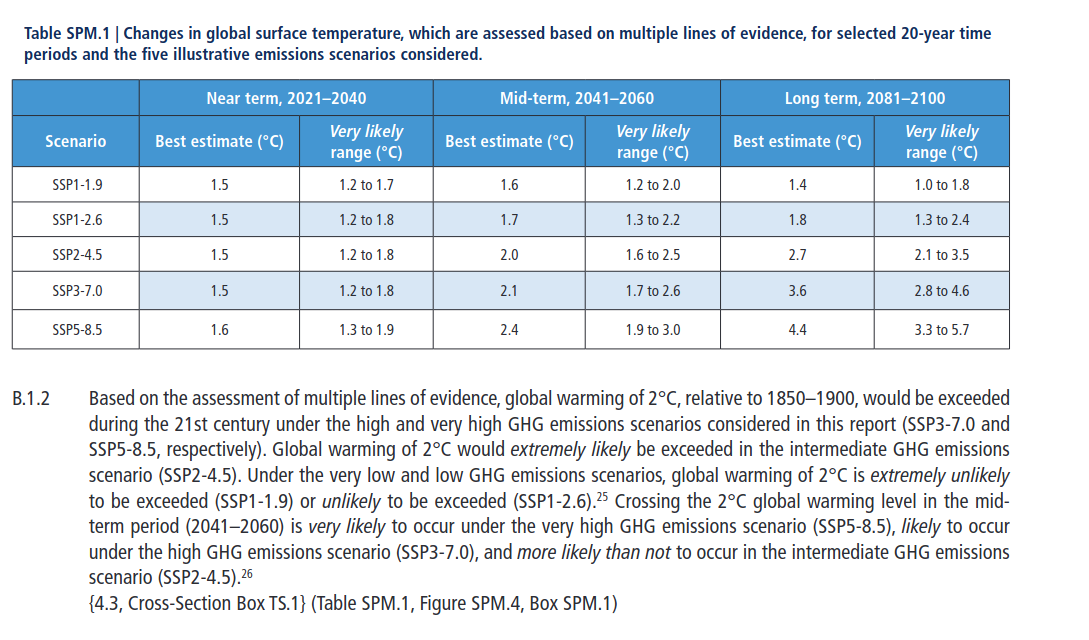
\includegraphics[width=0.7\textwidth]{fig/ipcc-table-explanation.png}
   \caption{Explanation based on the contents of a table}
   \label{fig:table-explanation}
\end{figure}